\graphicspath{{chapters/_resources/}}

\chapter{Genome instability}

\hypertarget{transcriptional-control-in-cancer}{%
\section{19- Transcriptional Control in Cancer}\label{transcriptional-control-in-cancer}}

\hypertarget{transcription-and-genome-instability}{%
\section{Transcription and genome instability}\label{transcription-and-genome-instability}}

\hypertarget{r-loops}{%
\subsection{R-loops}\label{r-loops}}

RNA is quickly displaced as soon as it emerges from Pol II; during transcription RNA-DNA hybrid structure is required, but it is \emph{transient}. It has been observed that RNA can re-hybridize with the template DNA forming \textbf{RNA:DNA hybrid} and \textbf{R-loop structures}. R-loop formation results from a competition between the nascent RNA and the non-template DNA strand to hybridize with the template strand.

\begin{figure}
\centering
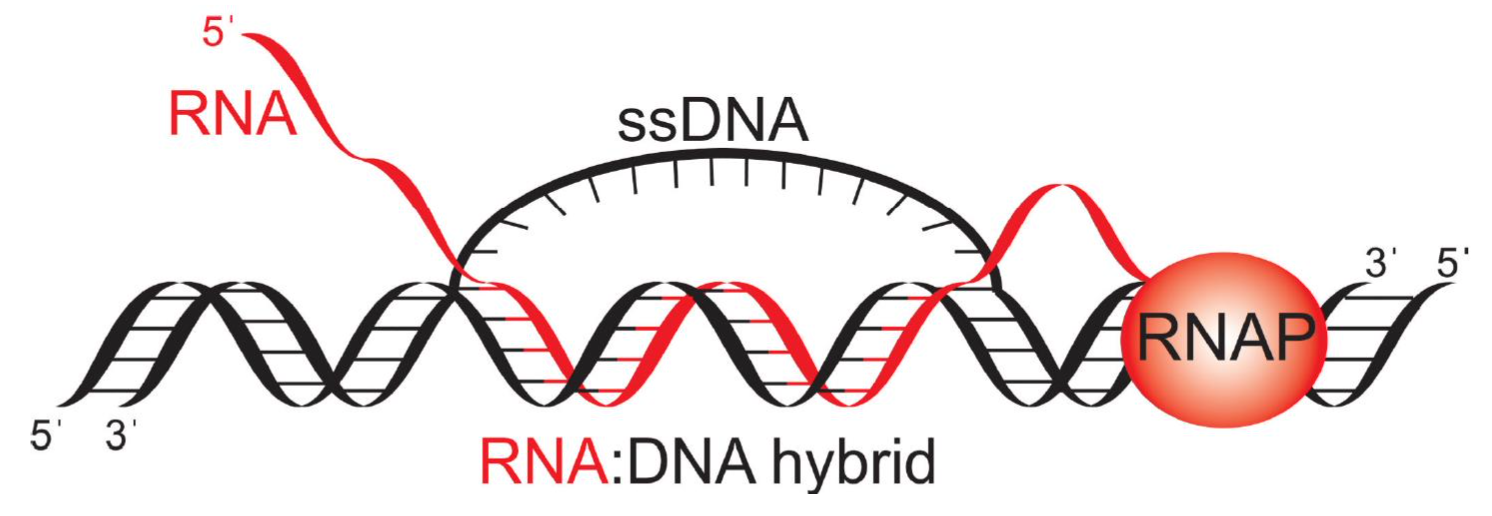
\includegraphics[width=0.5\textwidth]{../_resources/Screen_Shot_2022-11-23_at_09-53-33.png}
\caption{Hamperl and Cimprich, DNA Repair, 2014}
\end{figure}

Hamperl and Cimprich, DNA Repair, 2014

High G density in the non-template DNA strand promotes R-loops formation. RNA:DNA hybrids rich in RNA-G/DNA-C ratio are more stable than DNA:DNA duplex of the same sequence.

Transcription unwinding results in topological stress and generation of DNA supercoils.

\begin{itemize}
\tightlist
\item
  Positive toroidal supercoils: dsDNA is tightly packed
\item
  Negative toroidal supercoils: loose DNA, predisposition to RNA insertion.
\end{itemize}

Superhelical stress can favor, and be mitigated by, R-loops formation.

In highly transcribed genes we witness histone turnover, which is favored by negative supercoiling. R-loops formation inhibit nucleosomes redeposition weakening surrounding nucleosome-DNA contacts.

G-rich sequences and negative supercoiling can promote the formation of R-loops

In addition, to win competition with the non-template strand, the stability of the sequence is important → G-quadruplexes highly increase stability.

\textbf{G-quadruplexes:} 4 guanines interacting by hydrogen bonds (Hoogsteen) on the same plane (planar quartet). We can find parallel G4 or antiparallel G4 (based on the orientation of guanines).

R-loops are typically formed co-transcriptionally (cis) but formation in trans has been reported and expected e.g.~Cas9 pathway or ncRNA with unwinding promotion.

\hypertarget{r-loop-degradation}{%
\subsubsection{R-loop degradation}\label{r-loop-degradation}}

TREX complex: mediates transcript export for splicing and translation. If we remove THO subunit, we impair trex and formation of R-loops → limiting the amount of naked RNA in the cells prevents R-loops accumulation.

R-loops are also actively eliminated by specific enzymes:

\begin{itemize}
\tightlist
\item
  RNAse H1/2 recognize and degrade R-loops
\item
  RNA:DNA helicases e.g.~Sen1/SETX
\end{itemize}

\hypertarget{r-loop-recognition-and-distribution}{%
\subsubsection{R-loop recognition and distribution}\label{r-loop-recognition-and-distribution}}

\textbf{DRIP-seq:} The monoclonal S9.6 antibody revealed thousands of R-loop hotspots in human genome. R-loops can be found in:

\begin{itemize}
\tightlist
\item
  highly transcribed genes (as rate of transcription can influence loop formation for negative torsional stress)
\item
  telomeres: G-rich non-template strand, C-rich template strand
\item
  ORF: proposed function at termination sites for termination factor recruitment e.g.~chromatin remodeling.
\end{itemize}

! Pull down is performed after sonication, mechanic stress on DNA → bias. A good part of the signal could be coming from dsDNA. Over the years, improvements to the method were done e.g.~bisulphide for T→U, only finds RNA.

Endogenous R-loop structures are also detected by \textbf{R-ChIP}: a catalytically dead RNASEH enzyme can be expressed in cells, able to recognize but not degrade. We visualize R-loops endogenously. Bias: RNASE can be recruited on paused sites, the technique can only applied in cell lines.

R-ChIP and DRIP-seq experiments reveal R-loops enrichment at promoter regions and TSS. Approximately 60\% human promoters are associated with a CGI - CGI methylation generally associates with gene silencing.

R-loops form in human CpG island promoters with G-rich sequence at the non-template strand (GC skew) regulate DNA methylation.

Example of involvement of R-loops in transcription regulation.

\hypertarget{vim-antisense1}{%
\subsubsection{VIM-antisense1}\label{vim-antisense1}}

VIM is an intermediate filament in mesenchymal cells (EMT process). There is a presence of a CpG island. Usually with antisense the transcription of the sense collides due to sterical hindrance (overlapping). In this case, the antisense is polyadenylated and nuclear, while the sense is cytoplasmic. The expression of the antisense is associated with down-regulation of the sense gene. Depletion of VIM-AS1 causes downregulation of the VIM gene expression caused by methylation.

\begin{figure}
\centering
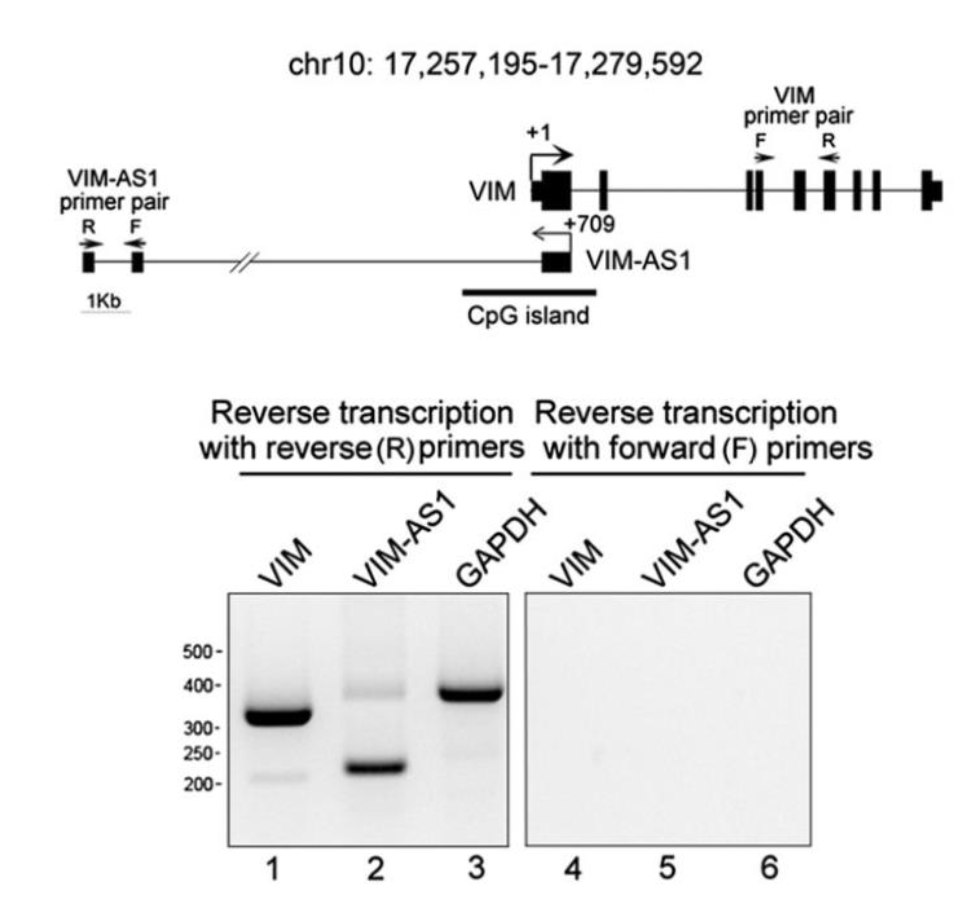
\includegraphics[width=0.5\textwidth]{../_resources/Screen_Shot_2022-11-23_at_10-18-00.png}
\caption{Screen Shot 2022-11-23 at 10-18-00.png}
\end{figure}

The two transcripts can be visualized through FISH with different fluorophores. By combining this technique with the inhibition of transcription VIM disappears, while VIM-AS1 is more stable. This could be due to the fact that it is engaged with a R-loop structure. The genomic region between the two TSSs shows GC skew sequences.

R-loop formation is dependent on the antisense transcript. RNaseH1 overexpression inhibits VIM and VIM-AS1 expression. R-loop structures promote VIM expression by impairing nucleosome occupancy and favoring the binding of transcription factors.

Expression of antisense and R-loop associate with open chromatin

By blocking R-loops or inhibiting VIM-AS1 at FNkB TF binding sites accessibility is reduced and the recruitment of the TF at the locus is impaired.

\hypertarget{main-findings}{%
\subsubsection{Main findings}\label{main-findings}}

\begin{itemize}
\tightlist
\item
  loop formation by antisense RNAs at CpG island containing promoters can impair DNA methylation at these promoter sequences
\item
  decrease nucleosome occupancy and favor binding of the transcription factor NF-kB to the promoter of Vimentin gene promoting transcription of the sense gene
\end{itemize}

R-loops can regulate gene expression by multiple mechanisms: repressing chromatin modifiers, activating chromatin modifiers and chromatin regulating complexes. They arise naturally and have multiple physiological effects e.g.~DNA repair, replication and gene expression, and are therefore tightly regulated. R-loops are generally transient and regulated by enzymatic activity; under certain conditions, R-loops become de-regulated and accumulate in cells.

\hypertarget{hottip-dependent-r-loop-formation-regulates-ctcf-boundary-activity-and-tad-integrity-in-leukemia}{%
\subsection{HOTTIP-dependent R-loop formation regulates CTCF boundary activity and TAD integrity in leukemia}\label{hottip-dependent-r-loop-formation-regulates-ctcf-boundary-activity-and-tad-integrity-in-leukemia}}

In vertebrates the Hox genes are located contiguously in clusters. Hox genes are expressed in a tightly regulated spatio-temporal manner during embriogenesis. They posses the homeobox domain and are divided into 4 clusters. The spatio-temporal expression is also observed in human primary fibroblast from different sites. 5C chromosome interaction highlights the presence of the \emph{posterior domain}. Differentiated cells (distal cells from limbs) have a distinct pattern with respect to proximal cells (from lung): in distal Pol II signal and H3K4me is observed in the first HOTTIP region, while the opposite patterns is present in proximal cells (HOTAIRM1 region at 3' → lncRNA interacting with chromatin remodelling complex).

HOTTIP stands for HOXA transcript at the distal tip. HOTTIP lncRNA stimulates the transcription of HoxA genes by enforcing H3K4me3 chromatin modification.

\begin{figure}
\centering
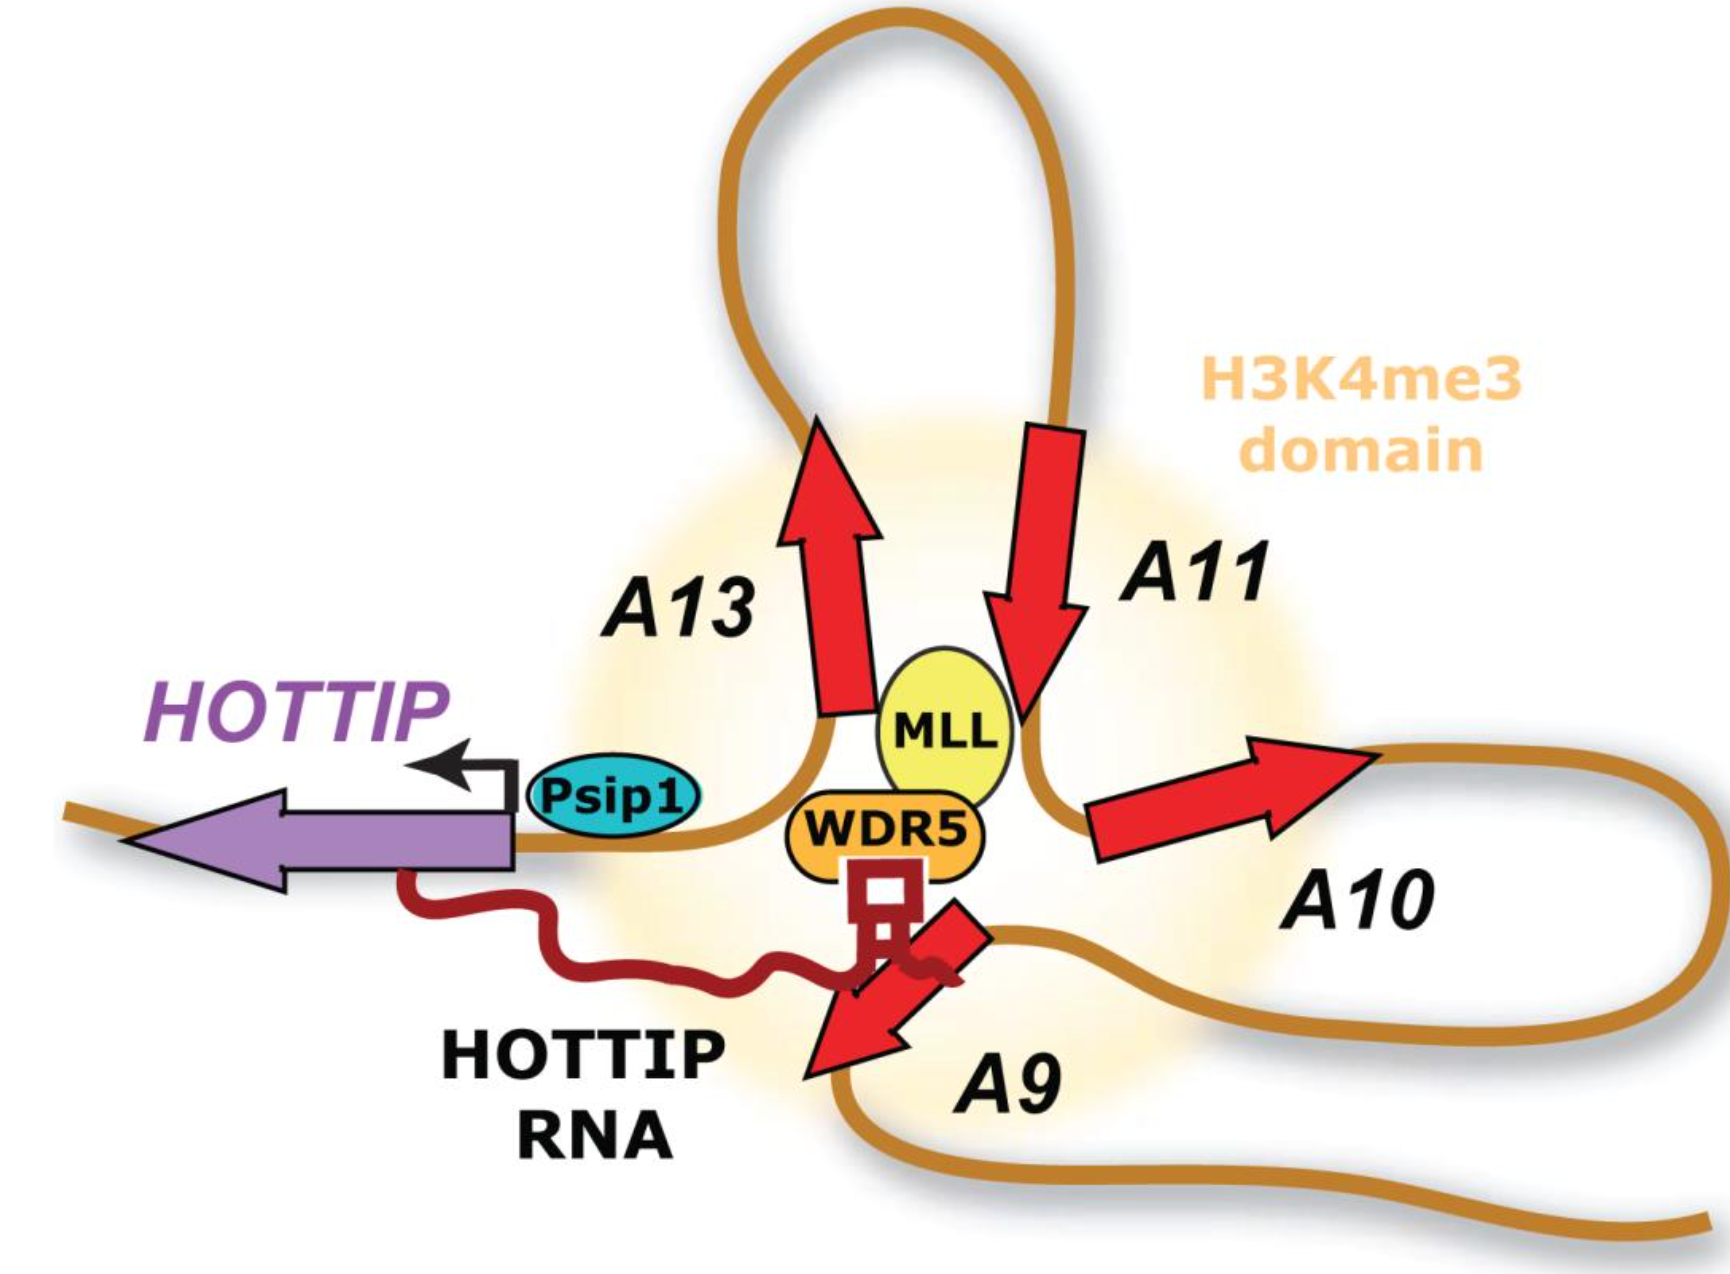
\includegraphics[width=0.5\textwidth]{../_resources/Screen_Shot_2022-11-25_at_11-49-03.png}
\caption{Screen Shot 2022-11-25 at 11-49-03.png}
\end{figure}

Chromosomal looping brings HOTTIP RNA in close proximity to the HOXA genes. HOTTIP lincRNA binds to and targets WDR5--MLL complexes to the HOXA locus, leading to transcription activation. The mutual interdependence between HOTTIP RNA and WDR5-MLL creates a positive feedback loop that maintains the ON state of the locus.

HOX genes are mutated or deregulated in different cancers and play active roles in tumorigenesis. HOXA genes are expressed in hematopoietic stem cells and progenitor cells while downregulated during differentiation. Abnormal HOXA gene activation is a common feature of acute myeloid leukemia (AML). HOXA9 and HOXA10 genes are frequently aberrantly activated in AML patients. Dysregulation of HOXA genes (e.g., HOXA9) is a driving mechanism for hematopoietic deregulation and leukemogenesis. Overexpression of HOXA9 is a poor prognostic marker in leukemia patients while its downregulation is a favorable predictor of AML patient outcome. The mechanisms regulating HOXA genes expression in AML patients is under investigation.

A transition from repressive to active chromatin is detected within the HOXA locus in AML patients. Among A7 and A9 we observe a sort of boundary, mainly regulated by insulator sequences → the CTCF binding site located between HOXA7 and HOXA9 genes may regulate the aberrant activation of the HOXA9-13 genes in AML cells.

Deletion of the CTCF binding site between HOXA7/9 genes (CBS7/9+/-) alters HOXA gene expression in AML cell lines. The homozygous deletion was incompatible with cell survival, so heterozygous was used. ChIP-seq analyses of CBS7/9+/- cells show altered chromatin structure in the HOXA9-13 domain but not in the HOXA1-7 locus, consistent with a loss of boundary function. 4C-seq data indicate decreased HOXA9 interaction with proximal genomic sites.

\textbf{CBS7/9+/- is important to regulate the chromatin structure and the expression of HOXA9-13 genes in AML cells}

Dysregulation of CBS7/9 boundary inhibits leukemic cell proliferation and prolongs survival time of transplanted NSG mice. In addition to the local effect on chromatin marks and structure, a significant number of dysregulated genes was observed e.g.~oncogenic pathways RUNX1, SOX involved in myeloid activation.

Attenuation of the chromatin boundary disrupts the active chromatin domain and perturbs oncogenic gene expression in AML, in part by disrupting the HOXA9 oncogenic pathway. The CBS7/9 boundary located at the edge of the TAD encompassing the posterior HOXA genes establishes and maintains aberrant chromatin signatures and expression of the posterior HOXA genes to facilitate myeloid leukemogenesis. The elimination of CTCF fosters the formation of aberrant protein.

\emph{Can a normal CTCF boundary be hijacked to control oncogenic chromatin domain and transcription profiles for leukemic transformation and progression?}

HOTTIP--/-- perturbs HOXA gene-mediated oncogenic transcription program, we observe oncogene downregulation. The KO is able to recapitulate the effect of CBS7/9 on HOXA. In wt AML cells we can identify the anterior and posterior domain, in KO cells we observe a change in the posterior domain.

HOTTIP lncRNA is aberrantly expressed in a subset of AML patients and cells. NPM1-mutated (NPM1C+)or MLL-rearranged (MLLr+) AML cases (n = 76) exhibited elevated levels of HOTTIP expression. Survival rate was inversely correlated with HOTTIP expression.

Activation of HOTTIP rescues the HOXA gene chromatin defects in the CBS7/9+/-- AML cells.

HOTTIP transgenic expression in hematopoiesis leads to AML-like disease and promotes hematopoietic transcription programs.

\hypertarget{conclusions}{%
\subsubsection{Conclusions}\label{conclusions}}

\begin{itemize}
\tightlist
\item
  HOTTIP expression alters HOXA genes containing TADs and HOXA genes expression
\item
  HOTTIP KO affects leukemic transcription program while HOTTIP overexpression leads to AML-like disease
\item
  HOTTIP is aberrantly expressed in AML patients
\end{itemize}

\hypertarget{hottip-lncrna-promotes-hematopoietic-stem-cells-self-renewal-leading-to-aml-like-disease-in-mice}{%
\subsection{HOTTIP lncRNA Promotes Hematopoietic Stem Cells Self-Renewal Leading to AML-like Disease in Mice}\label{hottip-lncrna-promotes-hematopoietic-stem-cells-self-renewal-leading-to-aml-like-disease-in-mice}}

CHIRP: reminds us of ChIP for crosslinking and sonication. Instead of using antibodies, they use specific probes for RNA of interest with tilling oligos (bp with different regions of the RNA, increased yield of the pull down). At the end of the protocol we obtain RNA.

HOTTIP interactome isolated from AML cells contains CTCF/cohesin complex and R-loop- associated proteins.

HOTTIP KO resulted in a in a significant reduction of R loops and HOTTIP binding sites, especially when cobound to CTCF.

No signal from GRO-Seq → HOTTIP KO disrupted CTCF and cohesin TAD boundaries containing AML oncogenes such as $\beta$-catenin (CTNNB1). At these boundary sites HOTTIP RNAs form R-loops in trans. HOTTIP-mediated R-loop formation directly contributes to CTCF boundary activity.

R-loops disruption at the CBS-u2 boundary site impairs proliferation of AML cells.

\hypertarget{transcriptional-control-in-cancer}{%
\section{20- Transcriptional Control in Cancer}\label{transcriptional-control-in-cancer}}

\hypertarget{transcription-and-genome-instability-ii}{%
\section{Transcription and genome instability II}\label{transcription-and-genome-instability-ii}}

\hypertarget{dna-damage}{%
\subsection{DNA damage}\label{dna-damage}}

Single stranded DNAs are more susceptible to chemical modifications, strand breaks, mutagen sensitivity and secondary structure than dsDNAs. Also dsDNA is undergoing spontaneous chemical modifications. Basically, any covalent bond in DNA molecule can be attacked by a water molecule. It has been estimated that there are thousands of spontaneous lesions in our cells e.g.~depurination (G→sugar phosphate) or deamination (C→U). Spurious methylation can occur in bases different from cytosine; when a RNA pol II passes through modified bases, we can observe a stall or the insertion of an erroneous base, leading to mutations. The addition of chemical groups occurs when bases react with oxygen species e.g.~guanine + adduct radical gives 8-hydroxyguanine.

\textbf{Base excision repair} (BER) pathway eliminates modified bases or depurinated nucleotides.

\begin{figure}
\centering
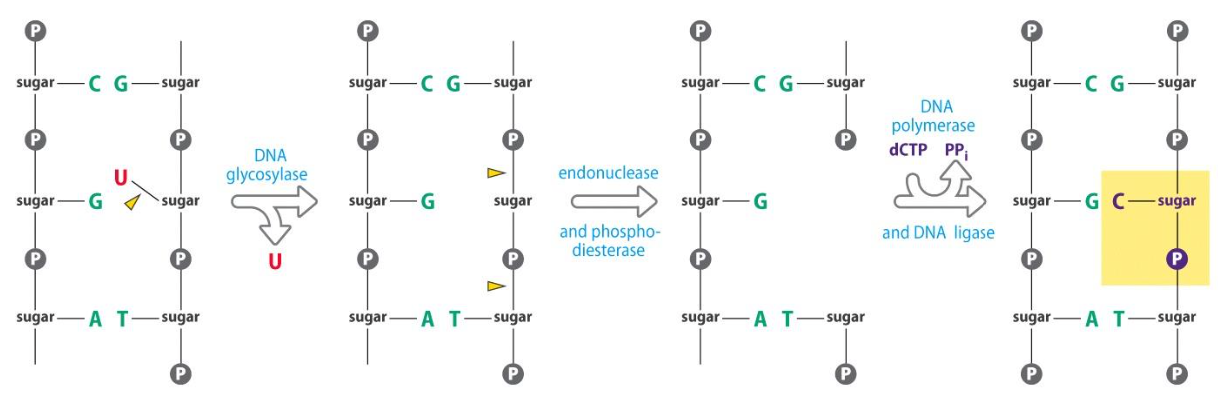
\includegraphics[width=0.5\textwidth]{../_resources/Screen_Shot_2022-11-30_at_08-49-05.png}
\caption{Base excision repair}
\end{figure}

Base excision repair

The chemical modification rate in oligonucleotides depends on cation concentration, pH, and other experimental conditions. Roughly 5\% of the genome can be occupied by R-loops.

\hypertarget{r-loop-modified-bases}{%
\subsubsection{R loop modified bases}\label{r-loop-modified-bases}}

Modified bases within R-loops that are not properly repaired form nicks and breaks (this step requires dsDNA) → replication and transcription stops. R-loops accumulation associates with genome instability due to the spontaneous base modifications occurring at ssDNA and the ensuing processing events leading to nicks and breaks.

\begin{figure}
\centering
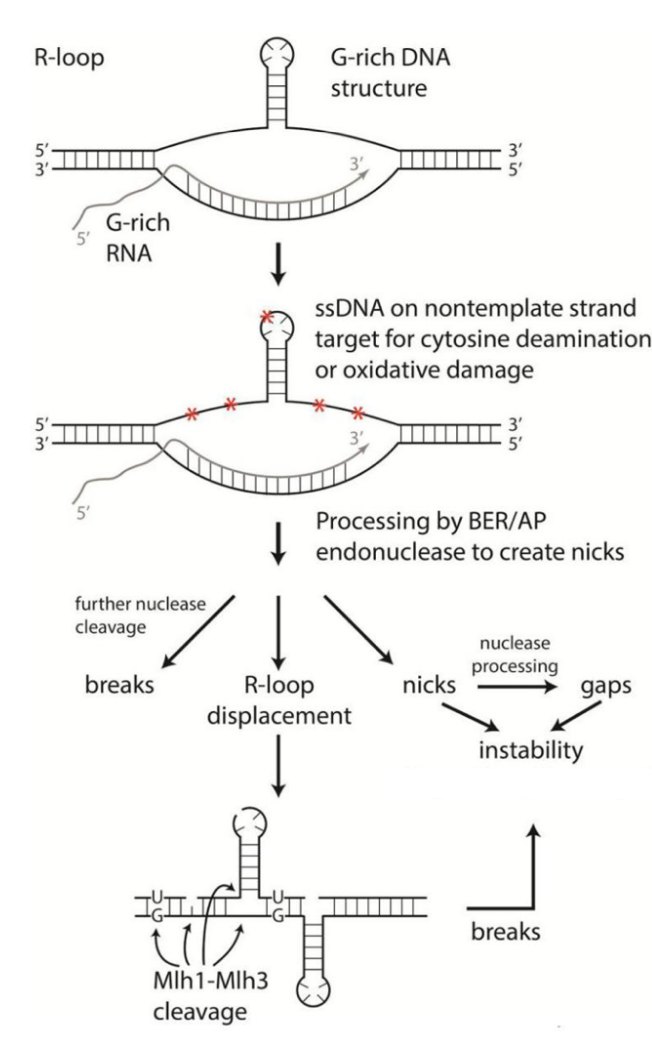
\includegraphics[width=0.5\textwidth]{../_resources/Screen_Shot_2022-11-30_at_08-51-07.png}
\caption{R loop repair}
\end{figure}

R loop repair

Thanks to R-loop displacement, BER can excite modified bases; this provokes a misaligned dsDNA, leading to breakages - especially if loops are hit by modifications - and genome instability.

R-loops can lead to nicks and breaks (DSBs) also due to the activity of the AID/APOBEC ****cytidine deaminases (catalyzed modifications). \textbf{Activation-induced cytidine deaminase} (AID) promotes somatic hypermutation and class switch recombination of immunoglobulin (Ig) genes in germinal center (GC) B cells. AID off-target activity has been implicated in malignant transformation of GC-derived B cell lymphomas.

C→U is meant to be, as cells want to induce mutation in a random manner to achieve hypervariability. In particular, several cancers are characterized by APOBEC signatures, which are a key source of mutation e.g.~chromosome instability in early breast and lung cancer evolution. Not only \emph{spontaneous} base modifications but also cytosine deamination catalyzed by \textbf{APOBECs} can lead to nicks and breaks within R-loops structures leading to genome instability.

\hypertarget{apical-kinases}{%
\subsection{Apical kinases}\label{apical-kinases}}

Cells have evolved the \textbf{DNA damage response} (DDR) in order to combat threats
posed by DNA damage. Breaks are sensed by apical kinases: \textbf{ATM}, \textbf{ATR} and \textbf{DNA-PKcs.} Phosphorylated serine or threonine residues followed by glutamine (S/T-Q) S/T-Q sites are present in ATM, ATR and DNA-PKcs for autophosphorylation. They all contain a kinase domain at the C-terminal. Cancer cells and immunodeficient cells (mutated in these genes) are more susceptible to radiation, since the recognition of ds breaks is impaired → radiotherapy would result in important side effects.

ATM, ATR and DNA-PKcs require specific co-factors for their recruitment to
damaged DNA. ATM is linked to a trimeric complex (MRN), where MRE11 is the endo/exo nuclease, RAD50 recognizes dsDNA and NBS1 is full of PPinteracting domain (ATM recruitment). ATR is recruited to dsbreaks when they are processed, so ssDNA bound by RPA (aspecific marker), bound by ATRIP co-factor.

\begin{figure}
\centering
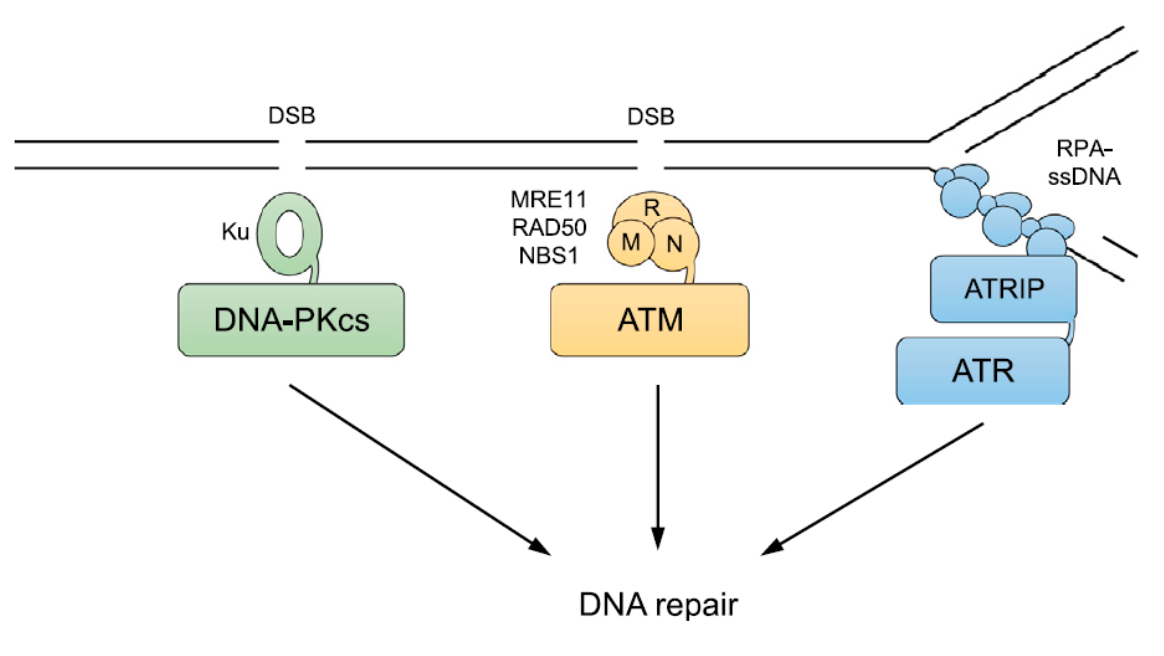
\includegraphics[width=0.5\textwidth]{../_resources/Screen_Shot_2022-11-30_at_09-11-05.png}
\caption{Apical kinases}
\end{figure}

Apical kinases

They are also involved in cell cycle control, DNA replication, transcriptional regulation and RNA metabolism. It orchestrates real cell response.

\textbf{DNA-PKcs} promotes NHEJ of DSBs: DNA-PKcs phosphorylation allows the recruitment of downstream NHEJ core factors, leading to DNA-end ligation by LIG4. This pathway is fast and can be used in all cell cycle phases.

ATM activation promotes a signaling cascade on damaged chromatin. MRN recruits ATM, which can phosphorylate hundreds of different targets, which are themselves kinases → kinase cascade. The first event is the phosphorylation of H2AX, leading to gamma H2AX marker for DNA damage. MDC1 is recruited and phosphorylation, additional MRN recruitment and feed-forward mechanism. Gamma H2AX can spread megabases, self sustaining cycle enhancing the reaction to ds break. TIP60 activates ATM through acetylation.

53BP1 is an effector of DNA damage response (reaction of the cell to ds break, enabling sensing) and DNA repair mechanism (fix the break) → NHEJ activation. Among the ATM targets we have BRCA1 (scaffold molecule and ubiquitinligase) and CtIP (endonuclease), which are phosphorylated → signal for the cell to activate homologous recombination (requires the sister chromatid, S phase only).

\begin{figure}
\centering
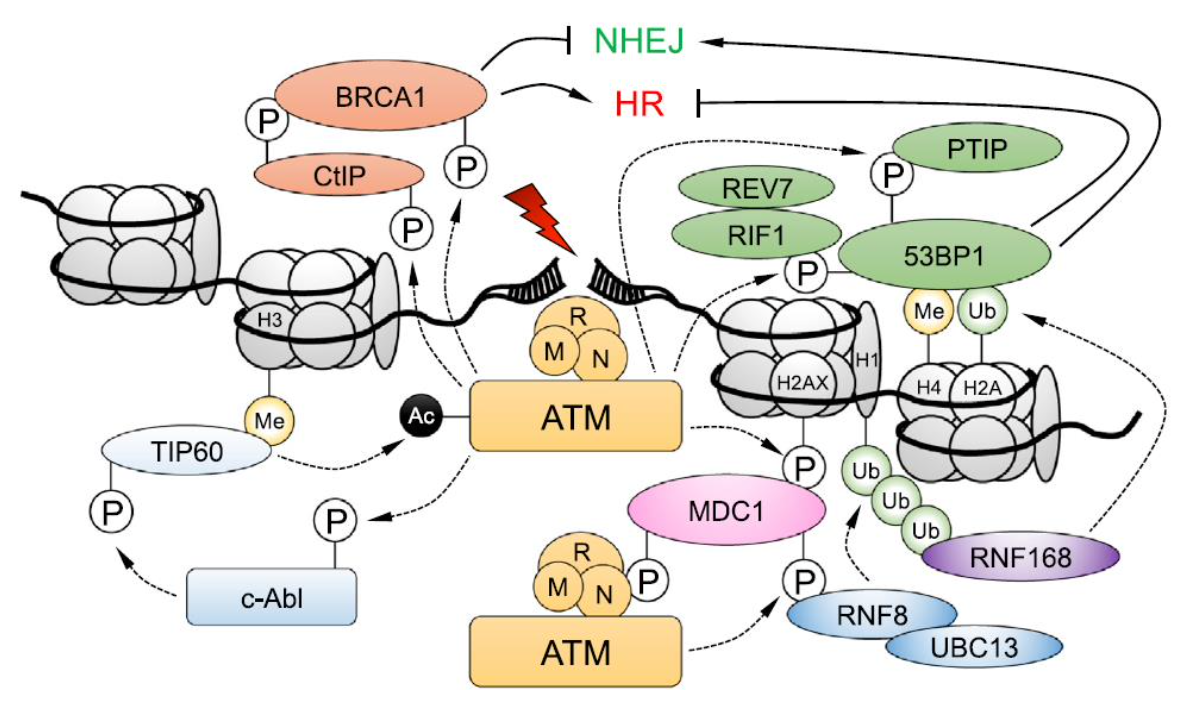
\includegraphics[width=0.5\textwidth]{../_resources/Screen_Shot_2022-11-30_at_09-16-55.png}
\caption{Blackford and Jackson, \emph{Mol Cell}, 2017}
\end{figure}

Blackford and Jackson, \emph{Mol Cell}, 2017

\textbf{BRCA1 and 53BP1 determine the choice of repair mechanism between NHEJ
and HR.} The decision between NHEJ and HR is also determined by several factors including cell cycle phase, chromatin state, genetics. NHEJ is ``error prone'' (but not in the classic pathway, alternative one), while homologous recombination is error free.

\begin{figure}
\centering
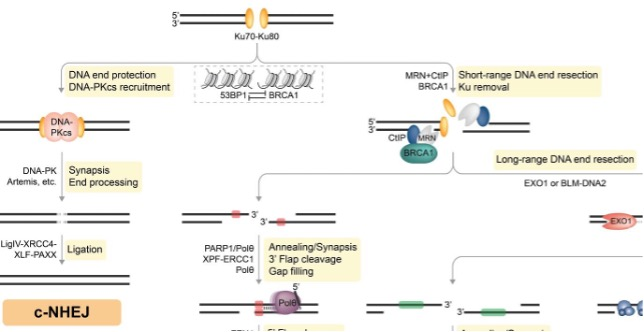
\includegraphics[width=0.5\textwidth]{../_resources/Picture1.jpg}
\caption{Trenner and Satori, Frontiers in Oncology 2019}
\end{figure}

Trenner and Satori, Frontiers in Oncology 2019

DNA damage response integrates regulation of the cell cycle, which is blocked in order to prevent mitosis. It is necessary to allow repair mechanism to act before resuming the cell cycle. Cell cycle is regulated by CHK2 (kinase phosphorylating CDK29) and p53.

The key signal for the cell in the context of repair comes from DNA ends; telomere mask chromosome ends from being recognized as double-strand breaks.

DNA damage response (DDR) involves DNA lesion recognition followed by a signaling cascade to promote DNA repair. The effectors lead to transient checkpoint, cellular senescence and apoptosis.

The roles o\textbf{f PARP1} (poly(ADP-ribose) polymerase 1) ****in detection and repair of DNA double-strand breaks are several. It is recruited to ds break and adds poly(ADP-ribose) chains. The recruitment of covalently and non-covalently modified proteins to site of DNA damage allows for repair of ssDNA nicks and breaks, sd breaks and chromatin modifications. PARP is also associated with ATM itself and is involved in HR, cNHEJ and aNHEJ. Although it is not the only activating mechanism of BRCA, it supports it to the break and lead to strand invasion and resolution.

Summarizing, defects in DSB repair e.g.~loss or Xrcc4, LIG4, BRCA1 lead to chromosome instability and accumulation of mutation → defective checkpoints, cancer.

\hypertarget{topoisomerases}{%
\subsection{Topoisomerases}\label{topoisomerases}}

Programmed ssDNA and dsDNA breaks occur during transcription. As we have mentioned, positive and negative torsional stress generate forces opposing the direction of pol II. Topoisomerase cleavage complexes (TOPcc) assemble at sites of topological stress. They are tightly regulated to minimize deleterious cleavage complexes - their activity is impeded by nucleosomes. They are recruited to chromatin via interaction with chromatin remodelling complexes (SWI/SNF), histone chaperones (FACT) and helicase enzymes (WRN).

TOP1 triggers SSBs or nicks, TOP2 induces DSBs. Both perform breakage in a controlled manner and once torsion is released they can exert ligation activity. During transcription TOP1 and TOP2 enzymes relieve positive supercoils while TOP1 and TOP3 counteract negative supercoils.

\hypertarget{a-topoisomerase-iib-mediated-dsdna-break-required-for-regulated-transcription}{%
\subsubsection{A topoisomerase IIb-mediated dsDNA break required for Regulated Transcription}\label{a-topoisomerase-iib-mediated-dsdna-break-required-for-regulated-transcription}}

Biotin-dUTP labelying by terminal deoxy .. → only if a break is present. Amplification of the promoter region and not of the ORF, signaling the presence of a break in the promoter leading to the recruitment of PARP. However the break is transient, after 10 minutes it disappears.

\begin{figure}
\centering
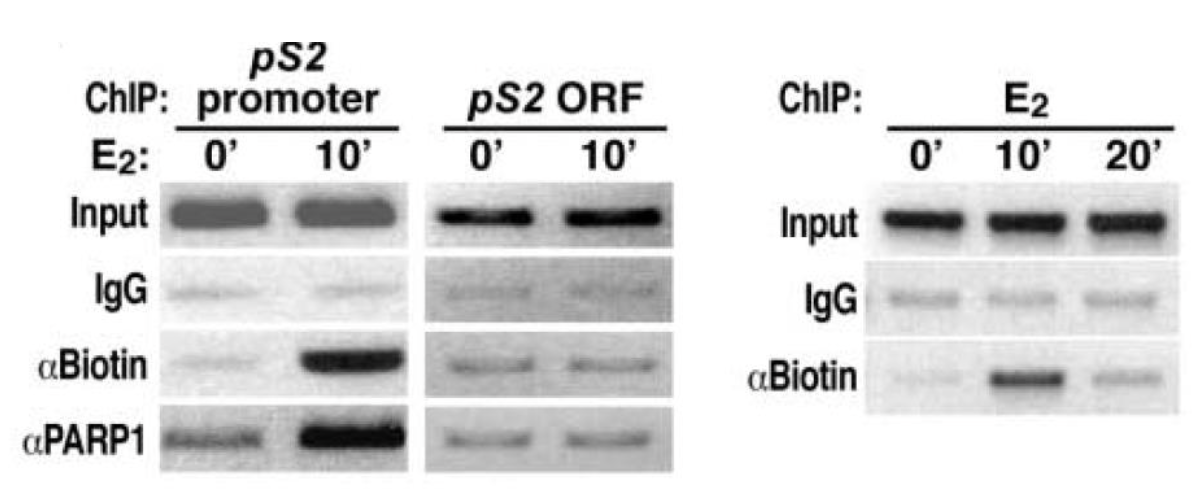
\includegraphics[width=0.5\textwidth]{../_resources/Screen_Shot_2022-11-30_at_10-03-17.png}
\caption{Screen Shot 2022-11-30 at 10-03-17.png}
\end{figure}

DSBs are induced transiently on the pS2 promoter upon estrogen treatment. Transcriptional activation associates with transient and local formation of DNA double strand breaks. TopoII$\beta$-mediated DSBs at the pS2 promoter is required for pS2 transcription. If we block topoisomerases, machinery for transcription is not recruited. The presence of DNAPK persists for a while after the resolution of the break, this does only mean that the signal is spreading.

TopoIIb/PARP-1 complex in nuclear receptor-mediated gene regulation TopoII mediated DSB and in PARP-1 activity serves as mechanism for gene transcription upon ligand or signal- dependent stimulation. PARP1 activity promotes removal of histone H1 from the ERE-containing nucleosome supporting transcription initiation.

\hypertarget{brca1}{%
\subsubsection{BRCA1}\label{brca1}}

Sometimes, patological topoisomerase 2 sites are observed. OP2 is required for ER-medited transcription. Occasional estrogen-induced pathological TOP2 occur with DSBs covalently associated with the enzyme. BRCA1 participates in resolving these structures promoting genome integrity. In the absence of BRCA1 estrogen exerts a genotoxic effect with accumulation of DSBs during cell divisions.

The roles of BRCA1 in the maintenance of genome integrity and regulation of transcription may be the key of its tissue specific tumor suppressor function.BRCA1 has an ubiquitinylase domain (RING) and a huge number of interacting proteins. BRCA1 drives a transcriptional program supporting differentiation of luminal progenitors to mature luminal cells. BRCA1 interaction inhibits ER$\alpha$ activity directly and by promoting mono-ubiquitination of ER$\alpha$. BRCA1 mutant progenitors are aberrantly proliferative and defective in differentiation giving rise to tumors of luminal origin. Cells with LOH in BRCA1 usually show basal-like tumor activity.

\hypertarget{stark-et-al.}{%
\subsubsection{Stark et al.}\label{stark-et-al.}}

24h estrogen treatment activates DNA damage response pathways and associates with DSBs in MCF7 cells. \textbf{Comet assay:} cells are lysate, nuclei as inserted in an agarose pad and placed under an electrophoretic chamber (no fragmentation): if there are ds breaks it will move a little bit, we will observe a ``comet'' signal. In 24 hours cells can cycle and perhaps this is not the same break as topoisomerase II. Long term estrogen treatment results in greater DDR activation than short term treatments.

DNA damage induced by long term estrogen treatment is replication dependent, the more the cell proliferate, the more the DNA damage response is activated. If a Cdc7 inhibitor, DNA damage response activation is impacted. Flavopiridol (inhibits Cdk9) results in Pol II elongation impairment, but does not affect replication.

Estrogen induces R-loops formation at ER responsive genes. The induction of R loop was depending on ER target genes. Gene responsive to estrogen are enriched in genomic rearrangements in breast tumors. Somatic mutation data from whole genome seq of 560 breast tumors determining whether the mutation sites are enriched in estrogen responsive loci.

Estrogen induced R-loops colocalize with DNA damage markers on chromatin. Proximity ligation assays suggest that estrogen induced R-loops occur on chromatin marked by DNA damage.

RNaseH expression reduces estrogen induced DNA damage. RNaseH expression reduces estrogen induced DSBs. R-loops may be involved in DNA damage induction DSBs formation in breast cancer cells upon estrogen treatment.

\textbf{Summary}

\begin{itemize}
\tightlist
\item
  Estrogen treatment induces replication and transcription dependent DNA damage
\item
  DNA damage and DSBs induced by estrogen stimulation are linked to R-loop formation at ER responsive genes
\item
  Breast cancer rearrangements are enriched at estrogen responsive loci where R-loops are detected upon estrogen treatment
\item
  Many DSBs that accumulate upon estrogen treatment are R-loops dependent
\item
  Estrogen stimulation leads to genome instability through R-loops formation and in a DNA
  replication dependent manner
\item
  Also highlights an «alternative» mechanism by which a transcriptional program plays a role in genome stability in cancer
\end{itemize}
